
\section{Enhancer Linking by Methylation/Expression Relationships (ELMER)}

Motivated by the discovery of transcriptional enhancers in tissue DNA methylation data \cite{berman2012ng}, and subsequent approaches to linking these enhancers to transcriptional targets using a chromQTL approach \cite{aran2013dna} (reviewed in \citeauthoronline{yao2015inferring}), \citeauthoronline{yao2015inferring} developed the the R/Bioconductor  \textit{ELMER} (Enhancer Linking by Methylation/Expression Relationships) package, a tool which infers regulatory element landscapes and transcription factor networks from cancer methylomes.

This tool combined DNA methylation and gene expression data from human tissues to infer multi-level cis-regulatory networks through several steps which included the identification of distal enhancer probes with significantly altered DNA methylation levels in primary tumor tissues compared to normal tissues, followed by the identification of putative target genes, and a comprehensive gene regulatory network analysis which combined transcription factor motifs at the altered enhancers with TF expression to identify the underlying master regulators. This approach identified several known and unknown master regulators in TCGA data, such as \sigla{GATA3}{GATA-binding protein 3} and \sigla{FOXA1}{Forkhead box protein A1} in breast cancer, and \sigla{P63}{tumor protein p63} and \sigla{SOX2}{Sex determining region Y-box 2} in squamous cell lung carcinoma \cite{yao2015inferring,silva2016tcga}.

Based on user feedback and a full review of the source code, we identified and implemented a number of software improvements, which are summarized in table \ref{tab:summary}: (i) The original package contained no standard data structure to handle multiple assays (DNA methylation, gene expression, and clinical data), which would be required for an integrative genomic data analysis. Recently, the Bioconductor team provided such a data structure through the \href{http://bioconductor.org/packages/MultiAssayExperiment/}{MultiAssayExperiment} package. (ii) All auxiliary databases (human TF list, classification of TF in families, gene annotation, DNA methylation annotation and motif occurrences within probe sites) used in the package were created and maintained manually, thereby making the upgrade process laborious; thus, we automated this process. (iii) The package was developed to analyze primary tumor tissue samples compared to normal tissues samples, thus not allowing arbitrary subgroups to be compared (for instance mutants vs. non-mutants, treated vs. untreated, etc.) (iv) Our original approach used known epigenomic markers for enhancers to constrain the genomic regions searched for differential methylation. However, this selection could limit our algorithm to identifying regulatory networks for tissue types that exist in the epigenomic databases; we found this constraint problematic, and thus now search \textit{all} distal regulatory regions without any such filter. (v) The function used to download data from The Cancer Genome Atlas (TCGA) data portal \cite{tomczak2015cancer} broke when the TCGA site was shutdown and its data transferred to The NCI's Genomic Data Commons (GDC) \cite{grossman2016toward}; we now have a more general data provider interface that supports GDC as the default provider. (vi) The package only supported data aligned to Genome Reference Consortium GRCh37 (hg19), and we now provide support for Genome Reference Consortium GRCh38 (hg38). (vii) There was no support to the recent HumanMethylationEPIC (EPIC) array. In addition to the specific improvements listed above, we substantially re-wrote most of the code to be more efficient and maintainable,  also most of the output plots generated were improved.

\begin{table}
\centering
\caption{Main differences between ELMER old version (v.1) and the new version (v.2)}
\label{tab:summary}
%{\def\arraystretch{2}\tabcolsep=10pt
\resizebox{\textwidth}{!}{%
\begin{tabular}{@{}m{4cm}m{6cm}m{6cm}@{}}
\toprule
\toprule
\multicolumn{1}{c}{\textbf{Features}} & \multicolumn{1}{c}{\textbf{ELMER Version 1}} & \multicolumn{1}{c}{\textbf{ELMER Version 2}}   \\ \midrule \midrule
Primary data structure      & mee object (custom data structure)   & MAE object (Bioconductor data structure) \\ \midrule
Auxiliary data      & Manually created   & Programmatically created \\\midrule
Number of human TFs       & 1,982 & 2,014 (UniProt database)    \\\midrule
Number of TF motifs      & 91    & 771  (HOCOMOCO v11 database)    \\\midrule
TF classification &  78 families         & 82 families and 331 subfamilies \newline(TFClass database, HOCOMOCO) \\\midrule
Analysis performed            & Normal vs tumor samples & Group 1 vs group 2   \\ \midrule
Statistical grouping            & Unsupervised only & Unsupervised or supervised using labeled groups   \\ \midrule
TCGA data source      & The Cancer Genome Atlas (TCGA) (not available)      & The NCI's Genomic Data Commons (GDC)     \\\midrule
Genome of reference      & GRCh37 (hg19)      & GRCh37 (hg19)/GRCh38 (hg38)          \\\midrule
DNA methylation platforms             & HM450  & EPIC and HM450            \\\midrule
Graphical User Interface (GUI)        & None  & TCGAbiolinksGUI     \\\midrule
Automatic report        & None  & HTML summarizing results    \\\midrule
Annotations      & None  & StateHub   \\
\bottomrule
\end{tabular}
}
%}
\end{table}

In this section, we present a new version of the R \textit{ELMER} package,
which addresses all the issues described above.

\subsection{Implementation}

Here we describe each of following analysis steps shown in figure \ref{fig:elmerworkflow}.

\begin{itemize}
    \item Organize data as a \textit{MultiAssayExperiment} object
	\item Identify distal probes with significantly different DNA methylation
   level when comparing two sample groups.
	\item Identify putative target genes for differentially methylated
   distal probes, using methylation vs. expression correlation
	\item Identify enriched motifs for each probe belonging
  to a significant probe-gene pair
	\item Identify master regulatory Transcription Factors (TF)
   whose expression associate with DNA methylation changes at multiple regulatory regions.
\end{itemize}


%\begin{landscape}
\tikzstyle{container} = [
    rectangle,
    draw,
    inner sep=0.2 cm,
    dashed
]
\tikzstyle{start} = [circle,
					 minimum size=2mm,
                     rounded corners=3mm,
					 very thick,
                     draw=green!50!black,
                     top color=green!50!black,
                     bottom color=green!50!black, 
                     text=white,
                     font=\tiny]

\tikzstyle{end} = [circle,
				  minimum size=2mm,
                  rounded corners=3mm,
                  very thick,draw=red!50!black, 
                  top color=red!50!black,
                  bottom color=red!50!black, 
                  text=white,
                  font=\tiny]

\tikzstyle{function} = [rectangle,
						minimum size=6mm,
                        rounded corners=3mm,
                        very thick,
                        draw=black!50, 
                        top color=white,
                        bottom color=white,
                        font=\itshape\footnotesize]

\tikzstyle{datain} = [
	rectangle, 
	rounded corners, 
    minimum width=3cm, 
    minimum height=0.5cm,
    text centered,
    font=\footnotesize, 
    draw=green!50!black, 
    fill=white, 
    text=black
]
                      
\tikzstyle{dataaux} = [
	rectangle, 
    rounded corners, 
    minimum width=3cm, 
    minimum height=0.5cm,
    text centered,
    font=\footnotesize,
    draw=orange, 
    fill=white, 
    text=black
]
                       
\tikzstyle{dataout} = [
	rectangle, 
	rounded corners, 
    minimum width=3cm, 
    minimum height=0.5cm,
    text centered,
    font=\footnotesize, 
    draw=blue, 
    fill=white, 
    text=black
]

% Pacakge labels
\tikzstyle{arrow} = [
	thick,
    ->,
    >=stealth,
    -latex',
    draw,
    rounded corners
]

\tikzstyle{labelelmer}=[
	rectangle,
    draw,
    fill=black!50!red,
    draw = black,
    minimum width=450pt,
    minimum height=1.5em,
    text=white,
    rotate = 90, 
    label={[rotate=90]center:\textcolor{white}{\textbf{ELMER package}}}
]

\tikzstyle{labeltcgabiolinks}=[
	rectangle,
	draw,
    fill=black!50!blue,
    draw = black,
    minimum width=420pt,
    minimum height=1.5em,
    text = green,
    rotate = 90, 
    label={[rotate=270]center:\textcolor{white}{\textbf{TCGAbiolinks/TCGAbiolinksGUI packages}}}
]


\tikzstyle{labelfuncivar}=[
	rectangle,
	draw,
    fill=black!20!orange,
    draw = black,
    xshift = -0.0cm,
    minimum width=480pt,
    minimum height=1.5em,
    text=white,
    rotate = 0, 
    label={[rotate=0]center:\textcolor{white}{\textbf{StateHub/StatePaintR/funcivar package}}}
]
\tikzstyle{labelgdc}=[
	rectangle,
	draw,
    fill=black!50!gray,
    draw = black,
    minimum width=167pt,
    minimum height=1.5em,
    text=white,
    yshift = 0.10cm,
    xshift = 0.1cm,
    rotate = 0, 
    label={[rotate=0]center:\textcolor{white}{\textbf{GDC database}}}
]
\tikzstyle{every annotation}=[fill=white, font=\sf \small, scale=0.5, text width=4cm, inner sep=2mm, text=black,draw = orange]


\begin{figure}[!ht]
\centering
  \resizebox{0.95\textwidth}{!}{%
\begin{tikzpicture}[node distance = 1.5cm, auto, shorten >=1pt,thick,font=\itshape\footnotesize]
\linespread{0.8}{
%\node (start) [start] {START};
\node (func1) [function, yshift = -0.5cm] {\textit{createMAE}};
\node [datain, right of=func1, yshift = 0.5cm, xshift = 2cm] (dna) {DNA methylation object};
\node [datain, right of=func1, yshift = -0.5cm, xshift = 2cm] (exp) {Gene expression object};
\node (out1) [dataout, below of=func1, yshift = -0.3cm,text width=3cm] {Multi Assay Experiment object};
\node (func2) [function, below of = out1] {get.diff.meth};
%\node (out2) [dataout, below of=func2, yshift = 0.3cm] {List of differently methylated probes};
\node (func3) [function, below of=func2] {GetNearGenes};
%\node (out3) [dataout, below of=func2, yshift = 0.3cm] {List of near genes for differently methylated probes};
\node (func4) [function, below of=func3] {get.pair};
%\node (out4) [dataout, below of=func4, yshift = 0.3cm] {List of pairs: differently expressed gene and differently methylated probes};
\node (func5) [function, below of=func4, yshift = -0.5cm] {get.enriched.motif};
%\node (out5) [dataout, below of=func5, yshift = 0.3cm] {List of enriched motifs};
\node (func6) [function, below of=func5] {get.TFs};
\node (func7) [function, below of=func6,yshift = -0.5cm] {TF.survival};
%\node (out5) [dataout, below of=func5, yshift = 0.3cm] {List of regulator};
\node [dataaux, left of=func5, xshift =-3cm] (elmerdata1) {Probes.motif};
%\node [dataaux, above of=elmerdata1] (enhancer) {enhancer};
\node [dataaux, left of=func6, yshift = 0.0cm, xshift =-3cm] (elmerdata2) {motif.relevant.TFs};
\node [dataaux, left of=func6, yshift = -1.0cm, xshift =-3cm] (elmerdata3) {human.TFs};
%\node (end) [end, below of=func7] {END};
\node (func8) [function, left of=func1,yshift = -3cm,xshift = -3cm] {get.feature.probe};
\node (probes) [datain, left of=func1,xshift = -3cm] {distal probes};
\node [dataaux, below of=func8] (tss) {ENSEMBL TSS};
\node [dataaux, below of=tss] (probesmetadata) {Probes metadata};


% funcvat
\node (funciVar) [function, below of=func7, xshift = 3cm, yshift = -1.4cm] {enrich.segments};
\node [dataaux, left of=funciVar,xshift = -2cm] (statehub) {Statehub tracks};
%\node [dataaux, left of=statehub,xshift = -2cm, yshift = 0.2cm] (encode) {ENCODE};
%\node [dataaux, left of=statehub,xshift = -2cm, yshift = -0.4cm] (roadmap) {ROADMAP};
%\node [dataaux, left of=statehub,xshift = -2cm, yshift = 0.8cm] (blueprint) {BLUEPRINT};
%\draw [arrow,dashed,draw=orange] (encode.east) -- (statehub.west);
%\draw [arrow,dashed,draw=orange] (roadmap.east) -- (statehub.west);
%\draw [arrow,dashed,draw=orange] (blueprint.east) -- (statehub.west);

\draw [arrow,dashed,draw=orange] (statehub.east) -- (funciVar.west);

\draw [arrow] (func4) -- ++(4.9,0) -- ++(0,-1) |- node {} (funciVar);

% Draw edges
%\path [arrow] (start) -- (func1);
\path [arrow,dashed,draw=green!50!black] (dna) |- (func1);
\path [arrow,dashed,draw=green!50!black] (exp) |- (func1);
\draw [arrow,dashed,draw=blue] (out1.west) -- ++(-.5,0) -- ++(0,-1) |- (func4.west);
\draw [arrow,dashed,draw=blue] (out1.west) -- ++(-.5,0) -- ++(0,-1) |- (func6.west);
\draw [arrow] (func1) -- (out1);
\draw [arrow] (out1) -- (func2);
\draw [arrow] (func2) -- node {} (func3);
\draw [arrow] (func3) -- (func4);
\draw [arrow] (func4) -- node {} (func5);
\draw [arrow] (func5) -- node {}(func6);
\draw [arrow] (func6) -- (func7);
%\draw [arrow] (func7) -- (end);
\draw [arrow,dashed,draw=orange] (elmerdata1) -- node {} (func5);
\draw [arrow,dashed,draw=orange] (elmerdata2.east) -- (func6.west);
\draw [arrow,dashed,draw=orange] (elmerdata3.east) -- ++(.5,0) -- ++(0,0.2) |- (func6.west);
%\draw [arrow,dashed,draw=orange] (enhancer.north) -- (func8.south);
\draw [arrow,dashed,draw=orange] (tss.north) -- (func8.south);
\draw [arrow,dashed,draw=orange] (probesmetadata.east) -- ++(.1,0) -- ++(0,0.2) |- (func8.east);
\path [arrow,dashed,draw=green!50!black] (probes) -- (func1);
\draw [arrow] (func8.north)  --  (probes);

% Containers
\node [container, 
       fit=(exp)(dna)(func1)(probes), 
       label={[font=\scriptsize,anchor=east] west:Data input}]
       (container1){};
\node [container, 
	   fit=(func2), 
       label={[font=\scriptsize,anchor=west,name=lfunc1] east:{\parbox[c]{4.0cm}{Identifying differentially\\ methylated probes}}}]
       (container2){};
\node [container, 
       fit=(func3)(func4), 
	   label={[font=\scriptsize,anchor=west,name=lfunc2] east:{\parbox[c]{4.0cm}{Identifying putative \\probe-gene pairs}}}]
       (container3){};
\node [container, 
 	   fit=(func5), 
       label={[font=\scriptsize,anchor=west] east:{\parbox[c]{4.0cm}{Motif enrichment\\ analysis}}}]
       (container4){};
\node [container, 
       fit=(func6), 
       label={[font=\scriptsize,anchor=west] south east:Identifying regulatory TFs}]
       (container5){};
\node [container, 
       fit=(elmerdata1)(elmerdata1), 
       label={[name=l1,font=\scriptsize,anchor=east] west:ELMER.data}]
       (container6){};
%\node[draw,text width=3cm, above of = elmerdata1]{ELMER.data};
\node [container, 
	   fit=(func8)(probesmetadata), 
	   label={[name=l3,font=\scriptsize,anchor=east] west:{\parbox[r]{2.0cm}{Select probes \\$\pm 2Kb$  distant \\ from TSS}}}]
       (container8){};

\node [container, 
       fit=(elmerdata2), 
       label={[name=l2,font=\scriptsize,anchor=east] west:TFClass database}]
       (container7){};
\node [container, 
	   fit=(elmerdata3), 
	   label={[name=l3,font=\scriptsize,anchor=east] west:Uniprot database}]
       (container8){};
\node [draw,  
       minimum height=450pt,
	   minimum width=450pt,
       fit=(l1)(exp)(dna)(elmerdata3)(l2)(lfunc1)(lfunc2)]
       (container9){};
\node at (container9.west) [labelelmer] {};
  
%------------------------------ TCGAbiolinks
\node (GDCprepare) [function, right of = func1, yshift =-1.3cm,xshift =8.8cm] {\textit{GDCprepare}};
\node (GDCdownload) [function, above of = GDCprepare,yshift =-0.4cm] {\textit{GDCdownload}};
\node (GDCquery) [function, above of = GDCdownload,yshift =-0.4cm] {\textit{GDCquery}};
\node (TCGAanalysesurvival) [function, right of = func7,xshift =7.8cm] {\textit{TCGAanalyse\_survival}};
\node (TCGAanalyzeEAcomplete) [function, right of = func4,yshift =0.4cm,xshift =7.8cm] {\textit{TCGAanalyze\_EAcomplete}};
\node (TCGAanalyzePathview) [function, right of = func4,yshift =-0.7cm,xshift =7.8cm] {\textit{TCGAanalyze\_Pathview}};
\node (TCGAvisualizeoncoprint) [function, right of = func4,yshift =-1.8cm,xshift =7.8cm] {\textit{TCGAvisualize\_oncoprint}};

\draw [arrow] (GDCquery) -- node {}(GDCdownload);
\draw [arrow] (GDCdownload) -- (GDCprepare);
\draw [arrow] (GDCprepare.west) -- ++(-0.3,0) -- ++(0,0.2) |- (dna.east);
\draw [arrow] (GDCprepare.west) -- ++(-0.3,0) -- ++(0,0.2) |- (exp.east);

\node (subtypeinfo) [dataaux, below of = GDCprepare,yshift =0.6cm] {Subtype information};
\node (molecularinfo) [dataaux, below of = subtypeinfo,yshift =0.6cm] {Molecular data};
\node (clinicalinfo) [dataaux,  below of = molecularinfo,yshift =0.6cm] {Clinical data};
\node (mafinfo) [dataaux, below of = clinicalinfo,yshift =0.6cm] {Mutation data};

\draw [arrow,dashed,draw=orange] (mafinfo.east) -- ++(0.5,0) -- ++(0,-0.2) |-    (TCGAvisualizeoncoprint.east);
\draw [arrow,dashed,draw=orange] (clinicalinfo.east)  -- ++(0.3,0) -- ++(0,0.2) |-   (GDCprepare.east);
\draw [arrow,dashed,draw=orange] (subtypeinfo.east)   -- ++(0.2,0) -- ++(0,0.2) |-   (GDCprepare.east);
\draw [arrow,dashed,draw=orange] (molecularinfo.east) -- ++(0.3,0) -- ++(0,0.2) |-  (GDCprepare.east);
\node [draw,  
       minimum height=420pt,
       minimum width=170pt, 
       xshift = 0.25cm,
       yshift = -0.25cm,
       fit=(TCGAanalyzeEAcomplete)(GDCquery)(TCGAanalysesurvival)(clinicalinfo)(subtypeinfo)](container10){};
\node at (container10.east) [labeltcgabiolinks] {};
\draw [latex'-latex',double] (TCGAanalysesurvival) --  (func7);
\draw [arrow] (func4.east)  -- ++(4.4,0) -- ++(0,0.2) |-  (TCGAanalyzeEAcomplete);
\draw [arrow] (func4.east)  -- ++(4.4,0) -- ++(0,-0.2) |-  (TCGAanalyzePathview);
\draw [arrow] (func4.east)  -- ++(4.4,0) -- ++(0,-0.2) |-  (TCGAvisualizeoncoprint);
\draw [arrow] (func6.east)  -|   (TCGAvisualizeoncoprint.south);
%------------------------------ 
\node [labelgdc, above of = GDCquery,xshift=-0.30cm,yshift=-0.05cm] (gdc) {};
\draw [latex'-latex',double] (GDCquery) --  (gdc.300);

\draw [draw,dashed] (gdc.188) |- (GDCdownload.west);
\draw [arrow,dashed] (gdc.188) |- (mafinfo.west);
\draw [arrow,dashed] (gdc.188) |- (clinicalinfo.west) ;
\draw [arrow,dashed] (gdc.188) |- (molecularinfo.west) ;
}

\tikzstyle{labelencode}=[
	rectangle,
	draw,
    fill=black!50!gray,
    draw = black,
    minimum width=150pt,
    minimum height=1.5em,
    text=white,
    yshift = 0.10cm,
    xshift = 0.1cm,
    rotate = 0, 
    label={[rotate=0]center:\textcolor{white}{\textbf{ENCODE database}}}
]
\tikzstyle{labelroadmap}=[
	rectangle,
	draw,
    fill=black!50!gray,
    draw = black,
    minimum width=150pt,
    minimum height=1.5em,
    text=white,
    yshift = 0.10cm,
    xshift = 0.1cm,
    rotate = 0, 
    label={[rotate=0]center:\textcolor{white}{\textbf{ROADMAP database}}}
]
\tikzstyle{labelblueprint}=[
	rectangle,
	draw,
    fill=black!50!gray,
    draw = black,
    minimum width=150pt,
    minimum height=1.5em,
    text=white,
    yshift = 0.10cm,
    xshift = 0.1cm,
    rotate = 0, 
    label={[rotate=0]center:\textcolor{white}{\textbf{BLUEPRINT database}}}
]

\node [draw,  
       minimum height=6.52em,
       minimum width=480pt, 
       xshift = 1.60cm,
       yshift = 0.05cm,
       fit=(funciVar)(funciVar)](containerFunciVar){};
\node at (containerFunciVar.south) [labelfuncivar] {};


\node [labelencode, right of = statehub,xshift=-8.20cm,yshift=-0.15cm] (encode) {};
\node [labelroadmap, below of = encode,xshift=-0.1cm,yshift=0.7cm] (roadmap) {};
\node [labelblueprint, above of = encode,yshift=-0.8cm,xshift=-0.1cm] (blueprint) {};
%\draw [latex'-latex',double] (encode.180) --  (containerFunciVar.0);
\draw [double,->] (encode.0) --  (statehub.180);
\draw [double,->] (roadmap.0) -- ++(1.4,0) |-   (statehub.180);
\draw [double,->] (blueprint.0) -- ++(1.4,0) |-  (statehub.180);
\end{tikzpicture}
  }%
  
  \caption[ELMER workflow]{ELMER workflow: ELMER receives as input a DNA methylation object, a gene expression object (a matrix or a SummarizedExperiment object) and a Genomic Ranges (GRanges) object with distal probes to be used as filter which can be retrieved using the \textit{get.feature.probe} function. The function \textit{createMAE}  will create a Multi Assay Experiment object keeping only samples that have both DNA methylation and gene expression data. Genes will be mapped to genomic position and annotated using ENSEMBL database \cite{doi:10.1093/database/baw093}, while for probes it will add annotation from \citeauthor{doi:10.1093/nar/gkw967} (\href{http://zwdzwd.github.io/InfiniumAnnotation}{http://zwdzwd.github.io/InfiniumAnnotation}) . This MAE object will be used as input to the next analysis functions. First, it identifies differentially methylated probes followed by the identification of their nearest genes (10 upstream and 10 downstream) through the  \textit{get.diff.meth} and  \textit{GetNearGenes} functions respectively. For each probe, it will verify if any of the nearby genes were affected by its change in the DNA methylation level and a list of  gene and probes pairs will be outputted from \textit{get.pair} function. For the probes in those pairs, it will search for enriched regulatory Transcription Factors motifs with the  \textit{get.enriched.motif} function. Finally, the  enriched motifs will be correlated with the level of the transcription factor through the \textit{get.TFs} function. In the figure green Boxes represents user input data, blue boxes represents output object, orange boxes represent auxiliary pre-computed data and gray boxes are functions.}
  \label{fig:elmerworkflow}
\end{figure}
%\end{landscape}

\subsubsection{Organization of data as a \textit{MultiAssayExperiment} object}

To facilitate the analysis of experiments and studies with multiple samples
the Bioconductor team created the \href{http://bioconductor.org/packages/SummarizedExperiment/}{\textit{SummarizedExperiment}} class \cite{huber2015orchestrating}, a data structure able to store data and metadata for a single experiment but not for data spanning several experiments for the same sample. To overcome this problem, recently, the MultiAssay SIG (Special Interest Group) created the \href{http://bioconductor.org/packages/MultiAssayExperiment/}{MultiAssayExperiment class} \cite{mae2017} a data structure to manage and preprocess multiple assays for
integrated genomic analysis. This data structure is now an input for all main functions
of \href{https://github.com/tiagochst/ELMER}{\textit{ELMER}} and can be generated
by the \textit{createMAE} function.


To perform \textit{ELMER} analyses, users need to populate a \textit{MultiAssayExperiment}
with a DNA methylation matrix or \textit{SummarizedExperiment} object from
\sigla{HM450}{HumanMethylation450 BeadChip} or \sigla{EPIC}{MethylationEPIC BeadChip} platform;
 a gene expression matrix or SummarizedExperiment object for the same samples;
 a matrix mapping DNA methylation samples to gene expression samples; and a matrix with sample metadata (i.e. clinical data, molecular subtype, etc.). If TCGA data are used, the last two matrices will be automatically generated.
If using non-TCGA data, the matrix with sample metadata should be provided with at least a column with a patient identifier and another one identifying its group which will be used for analysis, if samples in the methylation and expression matrices are not ordered and with same names, a matrix mapping for each patient identifier their DNA methylation samples and their gene expression samples should be provided to the \textit{createMAE} function.
Based on the genome of reference selected, metadata for the DNA methylation probes, such as genomic coordinates, will be added from   \href{http://zwdzwd.github.io/InfiniumAnnotation}{\citeonline{zhou2016comprehensive}};
and metadata for gene expression and annotation is added from ENSEMBL database \cite{yates2015ensembl} using \href{http://bioconductor.org/packages/biomaRt/}{biomaRt}
\cite{durinck2009mapping}.

\subsubsection{Selecting distal probes}
Probes from HumanMethylationEPIC (EPIC) array and Infinium HumanMethylation450 (HM450)
array are removed from the analysis if they have either internal SNPs close to the $3'$
end of the probe; non-unique mapping to the bisulfite-converted genome;
or off-target hybridization due to partial overlap with non-unique elements \cite{doi:10.1093/nar/gkw967}.
This probe metadata information is
included in \href{https://github.com/tiagochst/ELMER.data}{\textit{ELMER.data}} package,
populated from the source file at \url{http://zwdzwd.github.io/InfiniumAnnotation}
\cite{doi:10.1093/nar/gkw967}.
To limit ELMER to the analysis of distal elements, probes located in regions of $\pm2 kb$
around \sigla{TSSs}{transcription start sites} were removed.

\subsubsection{Identification of differentially methylated CpGs (DMCs)}

For each distal probe, samples of each group (group 1 and group 2) are ranked by
their DNA methylation beta values, those samples in the lower quintile (20\% samples
with the lowest methylation levels) of each group are used to identify if the probe is
hypomethylated in group 1 compared to group 2, using an unpaired one-tailed t-test.
The 20\% is a parameter to the \textit{diff.meth} function called \textit{minSubgroupFrac}. For the (ungrouped) cancer case, this is set to 20\% as in \citeonline{yao2015inferring}, because we typically wanted to be able to detect a specific molecular subtype among the tumor samples; these subtypes often make up only a
minority of samples, and 20\% was chosen as a lower bound for the purposes of
statistical power (high enough sample numbers to yield t-test p-values that could
overcome multiple hypothesis corrections, yet low enough to be able to capture
changes in individual molecular subtypes occurring in 20\% or more of the cases.)
This number can be set arbitrarily as an input to the \textit{diff.meth} function
and should be tuned based on sample sizes in individual studies. In the \textit{Supervised} mode,
where the comparison groups are implicit in the sample set and labeled,
the \textit{minSubgroupFrac} parameter is set to 100\%.
An example would be a cell culture experiment with 5 replicates of the untreated cell line,
and another 5 replicates that include an experimental treatment.

To identify hypomethylated \sigla{DMCs}{differentially methylated CpGs},
a one-tailed t-test is used to rule out the null hypothesis:
$\mu_{group1} \geq \mu_{group2}$, where $\mu_{group1}$ is the
mean methylation within the lowest group 1 quintile (or another percentile
as specified by the \textit{minSubgroupFrac} parameter) and $\mu_{group2}$
is the mean within the lowest group 2 quintile. Raw p-values are adjusted
for multiple hypothesis testing using the Benjamini-Hochberg method
\cite{benjamini1995controlling}, and probes are selected when they had
adjusted p-value less than $0.01$ (which can be configured using
the \textit{pvalue} parameter). For additional stringency, probes are only
selected if the methylation difference: $\Delta = \mu_{group1} - \mu_{group2}$
was greater than $0.3$. The same method is used to identify hypermethylated DMCs,
except we use the \textit{upper} quintile, and the opposite tail in the t-test is chosen.

\subsubsection{Identification of putative target gene(s)}

For each differentially methylated distal probe (DMC), the closest 10 upstream
genes and the closest 10 downstream genes are tested for inverse correlation between
methylation of the probe and expression of the gene. To select these genes,
the probe-gene distance is defined as the distance from the probe to the transcription
start site specified by the ENSEMBL gene level annotations \cite{yates2015ensembl} accessed via
the R/Bioconductor package \href{http://bioconductor.org/packages/biomaRt/}{biomaRt} \cite{durinck2009mapping,durinck2005biomart}. By choosing a constant number of genes to test for each probe, our goal is to avoid systematic false positives for probes in gene rich regions. This is especially important given the highly non-uniform gene density of mammalian genomes.
Thus, exactly 20 statistical tests were performed for each probe, as follows.

For each probe-gene pair, the samples (all samples from both groups) are divided into two
groups: the $M$ group, which consisted of the upper methylation quintile (the 20\%
of samples with the highest methylation at the enhancer probe), and the $U$ group,
which consists of the lowest methylation quintile (the 20\% of samples with the
lowest methylation.) The 20\% ile cutoff is a
configurable parameter \textit{minSubgroupFrac} in the \textit{get.pair} function.
As with its usage in the \textit{diff.meth} function, the default value of 20\% is
a balance, allowing for the identification of changes in a
molecular subtype making up a minority (i.e. 20\%) of cases, while also yielding
enough statistical power to make strong predictions. For larger sample sizes or
other experimental designs, this could be set even lower.

For each candidate probe-gene pair,
the Mann-Whitney U test is used to test the null hypothesis that overall gene
expression in group M is greater than or equal than that in group U.
This non-parametric test was used in order to minimize the effects
of expression outliers, which can  occur across a very wide dynamic range.
For each probe-gene pair tested, the raw p-value $P_r$ is corrected for multiple
hypothesis using a permutation approach as follows.
The gene in the pair is held constant, and \textit{x} random methylation probes are
chosen to perform the same one-tailed U test, generating a set of \textit{x} permutation
p-values $P_p$. We chose the x random probes only from among those that were
"distal" (farther than $2kb$ from an annotated transcription start site), in order
to draw these null-model probes from the same set as the probe being tested \cite{sham2014statistical}.
An empirical p-value $P_e$ value was calculated using the following formula
(which introduces a pseudo-count of 1):

\begin{equation}
	P_e = \frac{num(P_p \leq P_r)+ 1}{x+1}
\end{equation}

Notice that in the \textit{Supervised} mode, no additional filtering is
necessary to ensure that the $M$ and $U$ group segregate by sample group labels.
The two sample groups are segregated by definition, since these probes were
selected for their differential methylation, with the same directionality,
between the two groups (Figure \ref{fig:mode}).

\begin{figure}[h!]
\centering
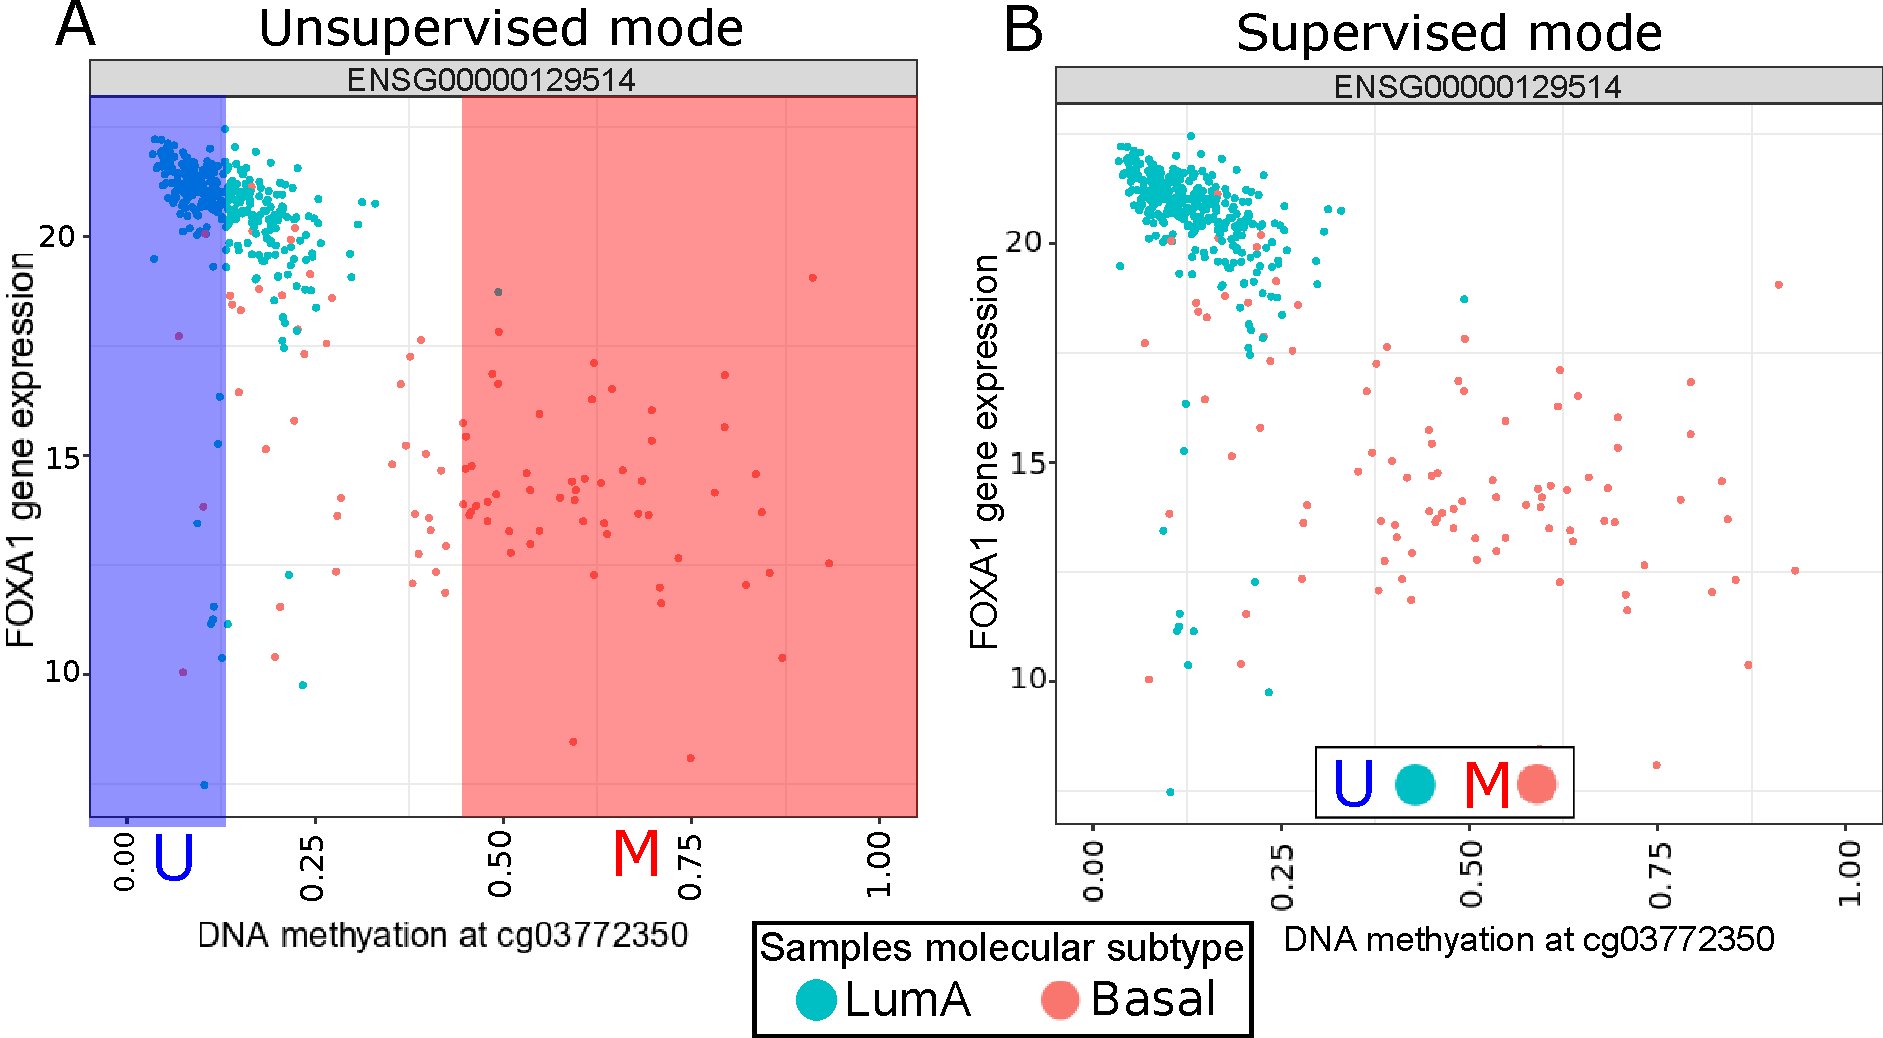
\includegraphics[width=1.0\textwidth]{images/mode_new.pdf}
\caption[Supervised vs unsupervised mode]{\label{fig:mode} Supervised mode maximizes statistical power.	Difference of groups $U$ and $M$ definition in \textit{supervised} and \textit{unsupervised} mode. A:  \textit{unsupervised} mode; when minSubgroupFrac argument is set to 40\%, the methylated group is defined as the highest quintile and the unmethylated group as the lowest quintile; B:  \textit{supervised} mode; methylated and unmethylated group are defined as one of the known molecular subtypes. For example, the unmethylated group is represented by all the LumA samples while the methylated group is represented by all the Basal samples. The t-test p-value achieved for the Unsupervised mode is $8.3E-25$, while the Supervised mode is : $1.43E-43$.}
\end{figure}




\subsubsection{Characterization of chromatin state context of enriched probes using StateHub}

Unlike version 1 of \textit{ELMER}, we now consider \textit{all} distal probes in the identification of regulatory elements. DNA methylation is known to affect several different classes of distal chromatin state element, including active enhancers, poised enhancers, super enhancers, and insulators. In order to provide a functional interpretation of the regulatory elements identified by \textit{ELMER}, we perform a chromatin state enrichment analysis of the probes within significant probe-gene pairs, using the \textit{statePaintR} tools from the \url{statehub.org} \cite{statepaintr}, along with the new \textit{FunciVar} package (in preparation on \burl{https://github.com/Simon-Coetzee/funcivar}). Enrichment of the putative pairs within chromatin states is calculated against a background model that uses the distal probe set that the putative pairs are drawn from. 

\subsubsection{Motif enrichment analysis}

In order to identify enriched motifs and potential upstream regulatory TFs, all probes with occurring in significant probe-gene pairs are combined for motif enrichment analysis. HOMER (Hypergeometric Optimization of Motif EnRichment) \cite{heinz2010simple} is used to find motif occurrences in a $\pm 250bp$ region around each probe, using HOCOMOCO (HOmo sapiens COmprehensive MOdel COllection) v11 \cite{kulakovskiy2016hocomoco} . Transcription factor (TF) binding models are available at \url{http://hocomoco.autosome.ru/downloads}. HOCOMOCO is the most comprehensive TFBS database and is consistently updated, marking an improvement over ELMER version 1. We have also improved the statistical analysis performed to use Fisher's exact test and Benjamini-Hochberg multiple hypothesis testing correction (see Supplemental Methods and Note). Importantly, we now characterize the Confidence Interval for the enrichment of each motif, and only select motifs that have an $FDR < 0.05$ \textit{and} where the lower bound of the Odds Ratio 95\% CI is greater than $1.1$ (specified by option \textit{lower.OR}). 

\subsubsection*{Identification of master regulator TFs}

When a group of enhancers is coordinately altered in a specific sample subset, this is often the result of an altered upstream \textit{master regulator} transcription factor in the gene regulatory network. \textit{ELMER}  identifies master regulator TFs corresponding to each of the TF binding motifs enriched from the previous analysis step.
For each enriched motif, \textit{ELMER} takes the mean DNA methylation of all distal probes (in significant probe-gene pairs) that contain that motif occurrence (within a $\pm 250bp$ region) and compares this mean DNA methylation to the expression of each gene annotated as a human TF. 
This step has been updated to work differently for the new \textit{Supervised} and \textit{Unsupervised} modes, using the same approach as described for the identification of putative target gene(s) step. This also can result in greater statistical power when using the \textit{Supervised} mode (see Supplemental Methods and Note for full details).

% I didn't understand this sentence. I thought the lower quintile was only for Unsupervised. Expect that for the \textit{supervised} mode we use the average methylation at all motif-adjacent probes to define the lower quintile.

% TO_SUPPLEMENTAL
%A statistical test is performed for each motif-TF pair, as follows. All samples 
%are divided into two groups: the M group, which consists 
%of the 20\% of samples with the highest average methylation at all motif-adjacent
%probes, and the U group, which consisted of the 20\%  of samples with the lowest 
%methylation. This step is performed by the \textit{get.TFs} function, which takes \textit{minSubgroupFrac} as an input parameter, again with a default of 20\%.
%For each candidate motif-TF pair, the Mann-Whitney U test is used to test 
%the null hypothesis that overall gene expression in group M is greater or equal 
%than that in group U. This non-parametric test was used in order to minimize the 
%effects of expression outliers, which can occur across a very wide dynamic range. 
%For each motif tested, this results in a raw p-value ($P_r$) for each of the human TFs.
As in ELMER version 1, all human TFs are ranked by their $-log_{10}(Pr)$ values, and those falling within the top 5\% of this ranking were considered candidate Master Regulators (see Figure \ref{fig:tfplot}, below). In addition to the top 5\% of all TFs, we also highlight all TFs from the same DNA binding domain family. In ELMER version 1, these families were defined by a hard-coded association file that was hand-curated. A major improvement of ELMER 2.0 is that we now use the classifications from the TFClass database \cite{wingender2013tfclass}, based on UniProt domains. Each TF is assigned to a family, as well as a more specific sub-family, of DNA binding domain proteins. For each significant motif, our output reports the most significant master regulator at both the family and sub-family level.




\subsection*{Data availability} % Optional - only if novel data or analyses are included
The TCGA data was downloaded from the NCI Genomic Data Commons (GDC) data portal \cite{grossman2016toward}
using TCGAbiolinks R/Bioconductor package \cite{colaprico2015tcgabiolinks,10.12688/f1000research.8923.2}.
Gene annotations were retrieved from ENSEMBL \cite{yates2015ensembl} database via biomaRt R/Bioconductor
package \cite{durinck2005biomart,durinck2009mapping}.
DNA methylation microarrays metadata were retrieved from \url{http://zwdzwd.github.io/InfiniumAnnotation} \cite{doi:10.1093/nar/gkw967}.
Transcription factor (TF) binding models can be downloaded at HOCOMOCO database (\url{http://hocomoco.autosome.ru/}) \cite{kulakovskiy2016hocomoco}.
The list of human TF can be accessed at \url{http://www.uniprot.org/}  \cite{apweiler2004uniprot}.
The classification of human transcription factors (TFs) can be viewed at \url{http://tfclass.bioinf.med.uni-goettingen.de/tfclass}  \cite{wingender2013tfclass}.

\subsection*{Software availability}

ELMER	source code  is available at \burl{https://github.com/tiagochst/ELMER}
and the auxiliary data files are available \burl{https://github.com/tiagochst/ELMER.data}.
\textit{ELMER} is available under the GNU General Public License version 3 (GNU GPL3).
